\documentclass[a4paper,11pt]{article}

\usepackage[utf8]{inputenc}
\usepackage[T1]{fontenc}
\usepackage[brazil]{babel}
\usepackage{amsmath,amssymb}
\usepackage{graphicx}
\usepackage{geometry}
\usepackage{listings}
\usepackage{xcolor}
\usepackage{booktabs}
\usepackage{pdfpages}
\usepackage{hyperref}

\geometry{a4paper, margin=2.5cm}

\definecolor{codebg}{rgb}{0.96,0.96,0.96}
\lstdefinestyle{matlabstyle}{
    language=Matlab,
    backgroundcolor=\color{codebg},
    basicstyle=\ttfamily\footnotesize,
    keywordstyle=\color{blue},
    commentstyle=\color{teal},
    stringstyle=\color{purple},
    numbers=left,
    numberstyle=\tiny\color{gray},
    stepnumber=1,
    breaklines=true,
    frame=single,
    showstringspaces=false,
    tabsize=2
}
\lstset{style=matlabstyle}

\title{Trabalho 2}
\author{Ettore Gabriel}
\date{\today}

\begin{document}

% ------------------------------------------------------------------
\begin{titlepage}
\centering
\vspace*{1cm}
{\large Universidade Tecnológica Federal do Paraná -- UTFPR}\\
{\large Campus Francisco Beltrão}\\[0.3cm]
{\large Disciplina: Análise de Sistemas Caóticos}\\
{\large Professor: Prof. Dr. Douglas da Costa Ferreira}\\[3cm]

{\Huge \textbf{Trabalho 2}}\\[0.5cm]
{\Large Modificações de Parâmetros nos Sistemas de EDOs}\\[0.3cm]
{\large Captação de Energia com Excitação Não-Ideal e Excitação Periódica}\\[3cm]

{\large Aluno: Ettore Gabriel}\\[0.3cm]
{\large \today}

\vfill
\end{titlepage}

% ------------------------------------------------------------------
\section{Introdução}

Este trabalho realiza, para cada um dos três sistemas de EDOs
apresentados na Aula 05 (\emph{Sistemas de EDOs para Captação de
Energia}), pelo menos uma modificação de parâmetro, comparando a
resposta dinâmica e a potência elétrica captada ($P=V_{rms}^2/R$, com
$R=0{,}1$) entre o caso \textbf{BASE} (parâmetros originais dos scripts
fornecidos) e o caso \textbf{MOD} (parâmetro alterado). Todas as
simulações usam Runge-Kutta de quarta ordem (\texttt{ode45}), passo de
amostragem $0{,}1$ e intervalo $t\in[0,\,2500]$.

\subsection{Sistema 1 -- Modelo Linear com Excitação Não-Ideal}
Neste modelo a viga piezoelétrica linear é excitada por um motor CC
desbalanceado (excitador não-ideal), com estados
$x_1$ (deslocamento), $x_2$ (velocidade), $x_3$ (ângulo do rotor do
motor), $x_4$ (velocidade angular do rotor) e $x_5$ (tensão elétrica):

\begin{align}
\dot{x}_1 &= x_2 \notag\\
\dot{x}_2 &= \frac{-\tfrac{1}{2}x_1 - 2\zeta x_2 + \chi x_5 + \mu x_4^2\cos x_3 + \mu\sin x_3\,(\alpha-\beta x_4)}{1-\mu\xi\sin^2 x_3} \notag\\
\dot{x}_3 &= x_4 \notag\\
\dot{x}_4 &= \xi\sin x_3\left(-\tfrac{1}{2}x_1 - 2\zeta x_2 + \chi x_5\right) + \mu\xi x_4^2\cos x_3\sin x_3 + \alpha - \frac{\beta x_4}{1-\mu\xi\sin^2 x_3} \notag\\
\dot{x}_5 &= -\kappa x_2 - \Lambda x_5 \notag
\end{align}

Parâmetros BASE: $\zeta=0{,}01$, $\chi=0{,}05$, $\kappa=0{,}5$,
$\Lambda=0{,}05$, $\mu=0{,}2$, $\xi=0{,}3$, $\beta=1{,}5$,
$\alpha=0{,}8$ (parâmetro de controle do torque do motor, faixa
indicada de $0{,}5$ a $5{,}0$). Condições iniciais: todos os estados
nulos, exceto $x_1(0)=1$.

\textbf{Modificação:} $\alpha:\,0{,}8 \rightarrow 3{,}0$ (motor com
torque/tensão de alimentação bem maior, dentro da faixa indicada).

\subsection{Sistema 2 -- Modelo Não-Linear com Excitação Não-Ideal}
Idêntico ao Sistema 1, exceto pela substituição do termo linear
$-\tfrac{1}{2}x_1$ pelo termo não-linear tipo \emph{Duffing}
$\tfrac{1}{2}x_1(1-x_1^2)$ nas equações de $\dot x_2$ e $\dot x_4$.
Parâmetros BASE idênticos ao Sistema 1, exceto $\alpha=4{,}0$.

\textbf{Modificação:} $\alpha:\,4{,}0 \rightarrow 1{,}0$ (redução do
torque do motor, favorecendo o motor "ficar preso" próximo à
ressonância -- efeito Sommerfeld).

\subsection{Sistema 3 -- Modelo Não-Linear com Excitação Periódica}
Viga não-linear (Duffing) excitada por uma base vibrante puramente
periódica $f\cos(\Omega t)$ (sem o motor CC), com estados $x_1$
(deslocamento), $x_2$ (velocidade) e $x_3$ (tensão elétrica):

\begin{align}
\dot{x}_1 &= x_2 \\
\dot{x}_2 &= \frac{1}{2}x_1(1-x_1^2) - 2\zeta x_2 + \chi x_3 + f\cos(\Omega t) \\
\dot{x}_3 &= -\kappa x_2 - \Lambda x_3
\end{align}

Parâmetros BASE: $\zeta=0{,}01$, $\chi=0{,}05$, $\kappa=0{,}5$,
$\Lambda=0{,}05$, $f=0{,}083$ (fixo) e $\Omega=0{,}8$ (parâmetro de
controle, faixa indicada de $0{,}4$ a $0{,}9$).

\textbf{Modificação:} $\Omega:\,0{,}8 \rightarrow 0{,}45$ (próximo do
limite inferior da faixa indicada no script original).

\section{Estabilidade Local (Autovalores)}

A Jacobiana de cada sistema foi calculada numericamente (diferenças
centrais, script \texttt{numjacobian.m}, já que o Symbolic Math Toolbox
não está disponível nesta instalação do MATLAB) e avaliada no ponto de
equilíbrio candidato igual à condição inicial de cada simulação
($x_1=1$, demais estados nulos). Como os parâmetros modificados
($\alpha$ e $\Omega$) não dependem dos estados, eles não alteram a
Jacobiana nesse ponto -- por isso os autovalores de BASE e MOD
coincidem em cada sistema (Tabela~\ref{tab:autovalores2}); as
diferenças de comportamento observadas nas simulações decorrem da
dinâmica forçada/acoplada, e não de uma mudança na estabilidade local
do ponto de equilíbrio analisado.

\begin{table}[h]
\centering
\caption{Autovalores no ponto de equilíbrio $x_1=1$, demais estados nulos.}
\label{tab:autovalores2}
\begin{tabular}{lll}
\toprule
\textbf{Sistema} & \textbf{Autovalores} & \textbf{Classificação} \\
\midrule
1. linear\_nao\_ideal & $-0{,}0112\pm0{,}7244i$;\ $-0{,}0476$;\ $-1{,}3923$;\ $-0{,}1077$ & Estável \\
2. nao\_linear\_nao\_ideal & $-0{,}0106\pm1{,}0123i$;\ $-0{,}0488$;\ $0{,}0000$;\ $-1{,}5000$ & Marg.\ estável \\
3. nao\_linear\_periodico & $-0{,}0106\pm1{,}0123i$;\ $-0{,}0488$ & Estável \\
\bottomrule
\end{tabular}
\end{table}

O Sistema 2 apresenta um autovalor nulo no ponto analisado (marginalmente
estável), coerente com o fato de esse ser justamente o modelo não-linear
em que, segundo a literatura de referência da disciplina, um dos
expoentes de Lyapunov é não-negativo -- ou seja, o sistema está no
limiar do comportamento caótico.

\section{Resultados e Discussão}

A Tabela~\ref{tab:resultados2} resume a potência elétrica captada em
regime permanente para os seis casos simulados.

\begin{table}[h]
\centering
\caption{Potência elétrica captada (regime permanente) -- BASE vs.\ MOD.}
\label{tab:resultados2}
\begin{tabular}{lccc}
\toprule
\textbf{Sistema} & \textbf{Potência BASE} & \textbf{Potência MOD} & \textbf{Variação} \\
\midrule
1. linear\_nao\_ideal        & $6{,}86\times10^{-2}$ & $1{,}10\times10^{-1}$ & $+61\%$ \\
2. nao\_linear\_nao\_ideal    & $8{,}93\times10^{-2}$ & $2{,}43\times10^{-2}$ & $-73\%$ \\
3. nao\_linear\_periodico     & $1{,}45\times10^{0}$  & $1{,}78\times10^{-2}$ & $-99\%$ \\
\bottomrule
\end{tabular}
\end{table}

\textbf{Sistema 1 (linear\_nao\_ideal):} aumentar o parâmetro de
controle do motor CC de $\alpha=0{,}8$ para $\alpha=3{,}0$ eleva o
torque disponível para o motor, aumentando a energia mecânica
transferida à viga e, consequentemente, a potência elétrica captada em
cerca de 61\%. O deslocamento em regime permanente também cresce (de
$0{,}20$ para $0{,}23$).

\textbf{Sistema 2 (nao\_linear\_nao\_ideal):} reduzir $\alpha$ de
$4{,}0$ para $1{,}0$ diminui fortemente o torque do motor. Nesse
modelo não-linear (Duffing) acoplado ao motor não-ideal, o torque menor
é insuficiente para "vencer" a ressonância do sistema mecânico
(efeito Sommerfeld/salto de energia), resultando em uma queda de
potência de cerca de 73\%, mesmo com amplitude de deslocamento em
regime praticamente inalterada -- ou seja, o motor gira, mas a energia
não é transferida de forma eficiente ao circuito elétrico.

\textbf{Sistema 3 (nao\_linear\_periodico):} reduzir a frequência de
excitação de $\Omega=0{,}8$ para $\Omega=0{,}45$ afasta a excitação da
faixa de maior resposta do sistema não-linear, provocando uma queda
drástica de potência (cerca de 99\%). Esse resultado evidencia a forte
sensibilidade da potência captada à frequência de excitação em sistemas
não-lineares, reforçando a importância de projetos de captadores que
mantenham a excitação próxima da faixa de ressonância do dispositivo.

\section{Scripts MATLAB}
\label{sec:scripts2}

\subsection{Sistema 1 -- Linear com Excitação Não-Ideal}
\lstinputlisting[caption={system\_linear\_nao\_ideal.m (BASE)}]{../scripts/system_linear_nao_ideal.m}
\lstinputlisting[caption={system\_linear\_nao\_ideal\_mod.m (MOD)}]{../scripts/system_linear_nao_ideal_mod.m}

\subsection{Sistema 2 -- Não-Linear com Excitação Não-Ideal}
\lstinputlisting[caption={system\_nao\_linear\_nao\_ideal.m (BASE)}]{../scripts/system_nao_linear_nao_ideal.m}
\lstinputlisting[caption={system\_nao\_linear\_nao\_ideal\_mod.m (MOD)}]{../scripts/system_nao_linear_nao_ideal_mod.m}

\subsection{Sistema 3 -- Não-Linear com Excitação Periódica}
\lstinputlisting[caption={system\_nao\_linear\_periodico.m (BASE)}]{../scripts/system_nao_linear_periodico.m}
\lstinputlisting[caption={system\_nao\_linear\_periodico\_mod.m (MOD)}]{../scripts/system_nao_linear_periodico_mod.m}

\subsection{Jacobiana Numérica e Autovalores}
\lstinputlisting[caption={numjacobian.m}]{../scripts/numjacobian.m}
\lstinputlisting[caption={autovalor\_aula2.m}]{../scripts/autovalor_aula2.m}

\subsection{Script Principal (Simulação e Geração dos Gráficos)}
\lstinputlisting[caption={run\_aula2.m}]{../scripts/run_aula2.m}

\section{Figuras}
\label{sec:figuras2}

Para cada um dos três sistemas, nos casos BASE e MOD, são apresentados:
o deslocamento, a velocidade e a tensão elétrica ao longo do tempo, o
retrato de fase tridimensional (tempo--deslocamento--velocidade) e o
retrato de fase bidimensional em regime permanente. A ordem das figuras
segue: Sistema 1 (BASE, depois MOD), Sistema 2 (BASE, depois MOD) e
Sistema 3 (BASE, depois MOD).

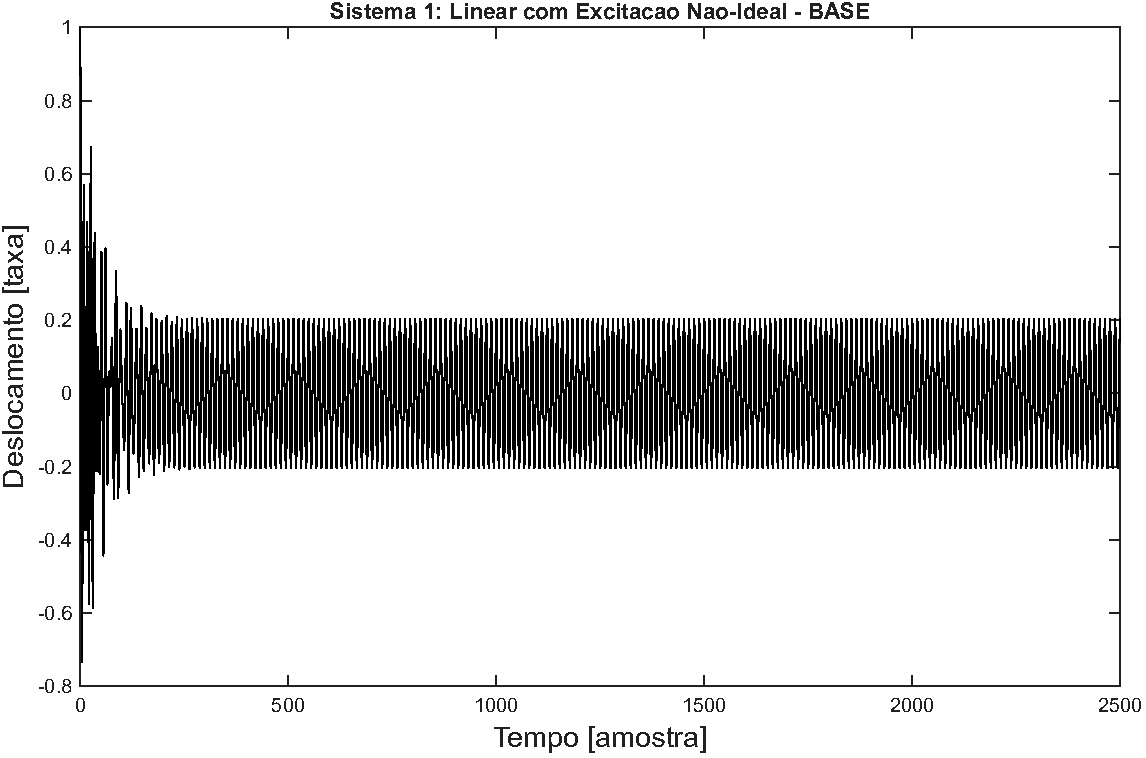
\includepdf[pages=-,pagecommand={},width=\textwidth]{../figuras/aula2_graficos.pdf}

\section{Conclusão}

As modificações realizadas em cada um dos três sistemas de EDOs
mostraram que o comportamento dos captadores de energia piezoelétricos
é altamente sensível aos parâmetros de excitação, seja ela não-ideal
(motor CC desbalanceado) ou puramente periódica. No modelo linear
não-ideal, aumentar o torque do motor aumentou a potência captada de
forma direta; já no modelo não-linear não-ideal, reduzir o torque
evidenciou o efeito Sommerfeld, no qual o sistema mecânico "trava"
próximo à ressonância e a conversão de energia se torna ineficiente.
No modelo não-linear com excitação periódica, afastar a frequência de
excitação da faixa de ressonância reduziu drasticamente a potência
captada. Esses resultados reforçam a importância do ajuste fino dos
parâmetros de excitação no projeto de dispositivos reais de captação de
energia por vibração.

\end{document}
